\documentclass{report}

% Language setting
% Replace `english' with e.g. `spanish' to change the document language
\usepackage[french]{babel}

% Set page size and margins
% Replace `letterpaper' with`a4paper' for UK/EU standard size
\usepackage[a4paper,top=2cm,bottom=2cm,left=3cm,right=3cm,marginparwidth=1.75cm]{geometry}

% Useful packages
\usepackage{amsmath}
\usepackage{bbold}
\usepackage{graphicx}
\usepackage[colorlinks=true, allcolors=blue]{hyperref}
\usepackage{breakcites}
\usepackage{color}
\newcommand{\com}[1]{\textcolor{olive}{#1}}
\newenvironment{comb}
    {\begin{color}{olive}
    }
    { 
    \end{color}
    }
\usepackage{tcolorbox}

\newcommand{\alh}[1]{\textcolor{teal}{#1}}


\title{Exploration de l'explicabilité de l'intelligence artificielle et de son application au traitement automatique de la langue naturelle} % une tentative à une heure tardive
\author{Marine Delvallez}

\begin{document}
\thispagestyle{empty}
    \setcounter{page}{0}
    \begin{center} 
        
\includegraphics[scale=0.4]{images/Logo Minerve_RVB.jpg}
        \hspace*{\stretch{1}}
        
\includegraphics[scale=0.2]{images/France_2030_Logo_rouge_bleu_transparent.png}
        \hspace*{\stretch{1}}
        
\includegraphics[scale=0.5]{images/LIFO.png} 
    \end{center}
    
    \vfill
    \begin{center}
        \rule{0.5\textwidth}{1pt}\\
        \vspace{0.5 \baselineskip}
        \huge \textbf{Projet individuel recherche Semestre 9 \newline M2 GPEx Minerve} \\
        \Large \textbf{Exploration de l'explicabilité de l'intelligence artificielle \newline et de son application au traitement automatique de la langue naturelle}\\
        \normalsize
        \rule{0.5\textwidth}{1pt}\\
        par \large Marine DELVALLEZ \normalsize \\
    
        \vspace{2cm}

        \begin{tabular}{llll}
            \emph{Jury} : & Thi-Bich-Hanh DAO &\emph{Tutrice de stage} : & Anaïs HALFTERMEYER\\
                          & Anaïs HALFTERMEYER &                        & \\
                          & Marie HENAULT
        \end{tabular}

        \vfill
        2 Septembre - 7 Janvier\\
        Année universitaire 2025-2026

    \end{center}

\tableofcontents


\chapter{Introduction}
    
    
    Le domaine de l'intelligence artificielle est en fort développement. De nouvelles méthodes d'apprentissage automatique sont régulièrement publiées et la performance de ces nouveaux modèles ne cesse de croître. L'intelligence artificielle cherche à faire adopter à une machine un comportement, une façon de répondre à un ensemble d'informations, qui soit rationnel et/ou au plus proche du comportement humain. Nous nous intéressons ici à l'apprentissage automatique (machine learning) et à l'apprentissage automatique profond (deep learning) qui sont des sous domaines de l'intelligence artificielle. \cite[Chap~19]{russell_intelligence_2021} défini l'apprentissage automatique comme le domaine de l'intelligence artificielle qui "construit un modèles à partir des données" en les observant. Les modèles sont à la fois des "hypothèses sur le monde" mais aussi des fonctions ou "procédures logicielles capables de résoudre certains problèmes". 
    Parmi ces problèmes, on retrouve les problèmes de classification comme la classification de spams ou la détection d'objets dans une image et les problèmes de régression comme la prédiction de prix d'un bien immobilier.
    %\alh{donner ici une transition un peu bateau donnant les exemples de tâche ou au moins les grandes classes de problèmes : classification, regression, partitionnement. Ou plus pragmatique : classification de spams, détection d'objet dans des images, ...}
    %L'augmentation de la performance des modèles en machine learning s'accompagne pour une partie d'entre eux d'une opacification de leur fonctionnement.
    Une façon intuitive d'automatiser la classification des spams est de définir des règles basées sur le contenu du mail comme la présence des mots "gratuit" et/ou "cliquez" ou l'adresse de l'expéditeur. Ces fonctionnements sont transparents pour l'humain : les règles sont intelligibles. Cependant, ces méthodes transparentes sont limitées et certains modèles et méthodes tels que les \emph{Random Forest} ou les réseaux de neurones sont plus avancées. Cette évolution qui apporte une augmentation des performances de ces systèmes engendre aussi une opacification de ces derniers qui perdent en transparence : 
    %\alh{c'est un peu violent : un truc du genre: la première intuition pour automatiser la classification de spam par exemple pourrait consister en l'édition de règles de repérage de mots tels que "gratuit", ou encore "cliquez", ce qui rend le système totalement transparent sur son fonctionnement puisque la règle appliquée est compréhensible pour un humain. Un tel système est transparent mais offre des capacités limitées, l'avènement de méthodes avancées en ML...}
    il devient de plus en plus dur de déterminer ce qui, lors du traitement d'une entrée, justifie le fait qu'un modèle aboutisse à la sortie obtenue. Ces modèles opaques sont souvent appelés \textbf{modèles boite-noire}. Cette perte de transparence des modèles pose problème pour certains usages. Dans les domaines de la santé ou de la défense, suivre la sortie obtenue par le modèle peut directement impacter la vie d'individus. Il n'est donc pas envisageable de faire confiance à un modèle dont on ignore le fonctionnement des processus de décision. De façon plus générale, le besoin de transparence a été pointé d'un point de vue juridique par la RGPD puis l'IAAct \cite{netter_regards_2019, iaact}. Tout personne subissant une décision (refus de dossier, sélection de profil,...) a droit à une justification de cette décision. Ainsi, toute personne décisionnaire utilisant des outils à base d'intelligence artificielle dans son processus de décision doit être en capacité de justifier les éléments fournis par l'outil dans ce cadre. %\alh{ce qui a permis de faire émerger un champs d'étude complet se préoccupant de la production de méthodes d'explicabilité dont l'objectif principal est de ...}
    Cela a permis de faire émerger un champ d'étude complet se préoccupant de la production de méthodes d'explicabilité dont l'objectif principal est d'exhiber les raisons faisant qu'un système obtient une certaine sortie. 
    Dans ce domaine, on appelle \textbf{explication} toute formulation intelligible et fidèle du fonctionnement d'un modèle d'intelligence artificielle. 
    
    Lorsqu'on s'intéresse aux modèles de langue et notamment aux modèles à base de Transformer \cite{vaswani_attention_2017, devlin_bert_2019, radford_improving_2018}, on retrouve les mêmes phénomènes. 
    %\alh{plutôt : notamment concernant les modèles à base transformer...}
    Ces nouveaux modèles sont de plus en plus puissants mais aussi de plus en plus opaques. La question de la transparence des processus de décision mis en \oe uvre au sein de ces modèles et systèmes se pose aussi. Les méthodes d'explicabilité standard 
    %\alh{"standard", "connues", ou encore "désormais classiques"} 
    s'appliquent bien dans ce contexte mais certaines sont en difficulté du fait des spécificités des technologies utilisées. Ainsi un besoin de méthodes spécifiques au modèles de langue a aussi émergé.
    


\chapter{Généralités}
    Dans ce chapitre, on introduit le vocabulaire utilisé ainsi que les différents concepts centraux de l'intelligence artificielle, ses outils et son explicabilité.
\section{Intelligence artificielle et modèles}
    Lorsqu'on construit un modèle d'intelligence artificielle, on cherche à assimiler les notions qui sous-tendent un problème. L'objectif est de construire un système capable d'effectuer une certaine tâche le plus rationnellement et/ou humainement possible. 
    
    Un modèle peut être vu de différentes manières. Lors de premières approches, on considère souvent un modèle comme une machine qui fourni une sortie ou qui a un comportement qui dépend des informations qui lui sont données. On peut se représenter cela comme une fonction qui à une entrée (\textbf{input}) associe une sortie (\textbf{output}). On parle alors de \textbf{système}. Dans ce cas, on s'intéresse aux domaines d'entrée (\textbf{environnement}) et de sortie associés au modèle ainsi que le comportement du système attendu (\textbf{spécification}). De façon plus générale, ces trois informations définissent la \textbf{tâche} attribuée au système. Par exemple, le dataset ImageNet \cite{russakovsky_imagenet_2015} propose des images étiquetées par l'animal qu'elles contiennent. Dans ce cas, l'ensemble des images d'animaux forme l'environnement, le domaine des sorties possibles est l'ensemble des étiquettes. C'est une tâche de classification.
    
    Une autre façon de considérer les modèles est de les voir comme des \textbf{représentations} d'un environnement. Dans ce cas, on ne s'intéresse plus aux entrées et sorties mais aux \textbf{paramètres} contenus dans le module et à ce qu'ils représentent. Ainsi, l'entraînement du modèle, qui n'était jusqu'ici qu'un protocole de construction d'une fonction, devient une procédure de capture d'un environnement. Avec cette approche du modèle en IA, la prédiction d'une sortie en fonction d'une entrée est considérée comme une \textbf{tâche tierce}. Le rôle principal d'un modèle vu ainsi est de \emph{représenter son environnement}. À partir de cette représentation, on peut extraire des informations qui permettent d'effectuer la tâche tierce. Pour cela, on ajoute parfois un composant supplémentaire à la sortie du modèle (souvent un petit réseau de neurone) pour obtenir un système capable d'exploiter la représentation de l'entrée proposée par le modèle. La Figure~\ref{fig:modele_systeme} illustre cette nuance. 
    
    \begin{figure}
        \centering
        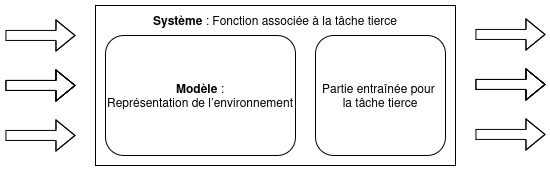
\includegraphics[width=\textwidth]{./images/PB_ModeleTacheTiers.drawio.jpg}
        \caption{Illustration de la distinction entre modèle et système}
        \label{fig:modele_systeme}
    \end{figure}

     Après son entraînement, lorsqu'on utilise un système ou un modèle, il \textbf{infère} la sortie à l'aide des données et de la représentation qu'il a apprise. Sa \textbf{prédiction} ne reflète pas nécessairement la réalité. 



\section{Explicabilité}
    \subsection{Définition d'explication}
    \label{ssec:def_expl}
        
        Lorsqu'on s'intéresse à l'explicabilité de l'intelligence artificielle, l'une des premières problémati\-ques rencontrée est la définition d'explication. Selon son utilisation, les attendus seront différents. Il en va de même pour le public auquel elle s'adresse (technicien, spécialiste ou grand public): sa forme dépend de la personne à qui elle est adressée.
        En explicabilité pour l'intelligence artificielle, on cherche à \emph{rendre humainement compréhensible les raisons pour lesquelles un modèle effectue une certaine prédiction} \cite{garouani_investigating_2024, bell_its_2022}. On estime la compréhension pour un humain par sa capacité à anticiper ou justifier la prédiction \cite{bell_its_2022}. Ainsi, une explication correspond à \emph{tout support ou expression rendant compte le plus fidèlement possible des processus de décision d'un modèle dans une forme la plus humainement intelligible possible}.
        
        Il ne faut pas confondre explicabilité et interprétabilité de l'intelligence artificielle. Un modèle est \textbf{interprétable} si il est possible pour un humain de comprendre les mécanismes de décision mis en \oe uvre par le modèle lui-même \cite{garouani_investigating_2024, gilpin_explaining_2019}. Du fait de cette contrainte de transparence du raisonnement du modèle, certains auteurs n'incluent dans cette catégorie que les arbres de décision, les modèles linéaires et ceux à base de listes de règles \cite{bell_its_2022}. Ainsi l'interprétabilité peut être vue comme le \emph{secteur du l'apprentissage automatique qui construit des modèles intrinsèquement humainement interprétables} \cite{rudin_stop_2019}. Là où l'explicabilité cherche \emph{pourquoi} le modèle produit une sortie ou une autre, l'interprétabilité va chercher \emph{comment} cette sortie est obtenue et construire des modèles pour lesquels il est possible de répondre à cette question. Par exemple, une interprétation pour un classifieur de spams fonctionnant avec des règles est de dire qu'on sait que les mails contenant les mots "gratuit" et "cliquez" seront classés comme spams. On fourni une verbalisation de la règle contenue dans le modèle. À contrario, une explication pour cet exemple peut être de dire que le mail est classé spam car la majorité des mails contenant à la fois les mots "gratuit" et "cliquez" ont aussi étés classés de cette façon par le système. Par conséquent, un modèle interprétable sera considéré comme explicable par la plupart des auteurs là où les modèles non interprétables peuvent aussi être expliqués.
        
        Au delà de la nuance entre les causes d'un phénomène et les mécanismes qui l'animent, les exigences qu'il est possible d'avoir envers les explications peuvent être très variables. Dans le cas de la classification d'images, \cite{chefer_transformer_2021} propose de considérer la capacité d'une explication à pointer l'élément correspondant à la classe dans l'image (une "carte de pertinence" met en évidence le chien sur l'image étiquetée par "chien"). Ce format d'explication est illustré dans la Figure~\ref{fig:carteinfluence} Si le fait de reconnaître et être capable de désigner l'objet important dans une image être un moyen pertinent dans le processus de décision, il peut aussi être intéressant de prendre en compte le contexte dans lequel se trouve l'objet. Par exemple, \cite{elguendouze_explainable_2024} met en évidence se type de comportement dans le contexte du sous-titrage d'images. Par exemple, si les images d'éléphant de la base de données sont toujours des images d'éléphant dans un milieux aride, le modèle peut considérer le milieu aride comme un indicateur en faveur de la présence d'un éléphant. \\
        Un autre format courant d'explication est d'attribuer une indication de l'importance de chaque composant de l'entrée. Elle prend souvent la forme d'un coefficient réel. 
        
    \begin{figure}
        \parbox{7cm}{%
        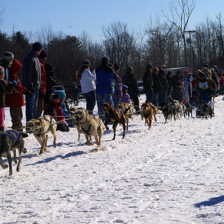
\includegraphics[width=0.3\textwidth]{images/37_orig.png}
        }
        \qquad
        \begin{minipage}{7cm}%
        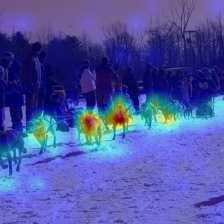
\includegraphics[width=0.64\textwidth]{images/37_grad_LRP.png}
        \end{minipage}%
        \caption{Image et explication de la classification "Chien" sous forme de "carte d'influence"}
        \label{fig:carteinfluence}
    \end{figure}

    
    \subsection{Les temps de l'explicabilité}
        Il existe différents temps au cours de la vie d'un modèle d'apprentissage automatique durant lesquels ont peut chercher à expliquer son fonctionnement. Au cours de la construction d'un modèle et de son entraînement, on peut chercher à le rendre plus transparent en travaillant sur les données, l'architecture du modèle ou la fonction d'apprentissage par exemple. On parle d'\textbf{explicabilité by-design}. Une fois un modèle prêt à être utilisé, avant ou au cours de son déploiement, on peut chercher à expliquer son fonctionnement en observant son comportement sur différentes entrées ou en essayant d'analyser les paramètres du modèle. On appelle cela l'\textbf{explicabilité post-hoc}. La Figure \ref{fig:VieModeleTempsXAI} illustre ces différents temps dans la vie d'un modèle.
        
        \begin{figure}
            \centering
            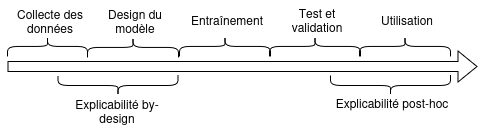
\includegraphics[width=\textwidth]{./images/VieModele-TempsXAI.png}
            \caption{Temps pour l'explicabilité dans la vie d'un modèle}
            \label{fig:VieModeleTempsXAI}
        \end{figure}



\chapter{Des modèles}
    Le secteur de l'apprentissage profond possède une grande diversité de modèles allant des simples réseaux de neurones profonds (DNN) jusqu'à des architectures plus complexes telles que les Long-Short-Term Memory (LSTM) en passant par des modèles plus spécialisés (CNN). Dans ce chapitre, on se concentre sur une autre famille d'architectures : le modèle Transformer et ceux qui s'en inspirent.

\section{Le modèle Transformer}
    
    Le modèle Transformer est introduit pour la première fois par \cite{vaswani_attention_2017}.  Comme on peut le constater dans la Figure~\ref{fig:transformer}, cette architecture n'utilise pas les outils utilisés à cette période tels que les RNN et LSTM mais repose exclusivement sur le \emph{mécanisme d'attention} (voir sous-section \ref{ssec:mecattention}) qui est l'élément central de cette architecture conséquente. \\
    Par la suite, plusieurs modèles se sont basés sur cette architecture faisant du mécanisme d'attention et du Transformer des éléments centraux du secteur de l'apprentissage profond \cite{lin_survey_2022}.
    
    \begin{figure}
        \centering
        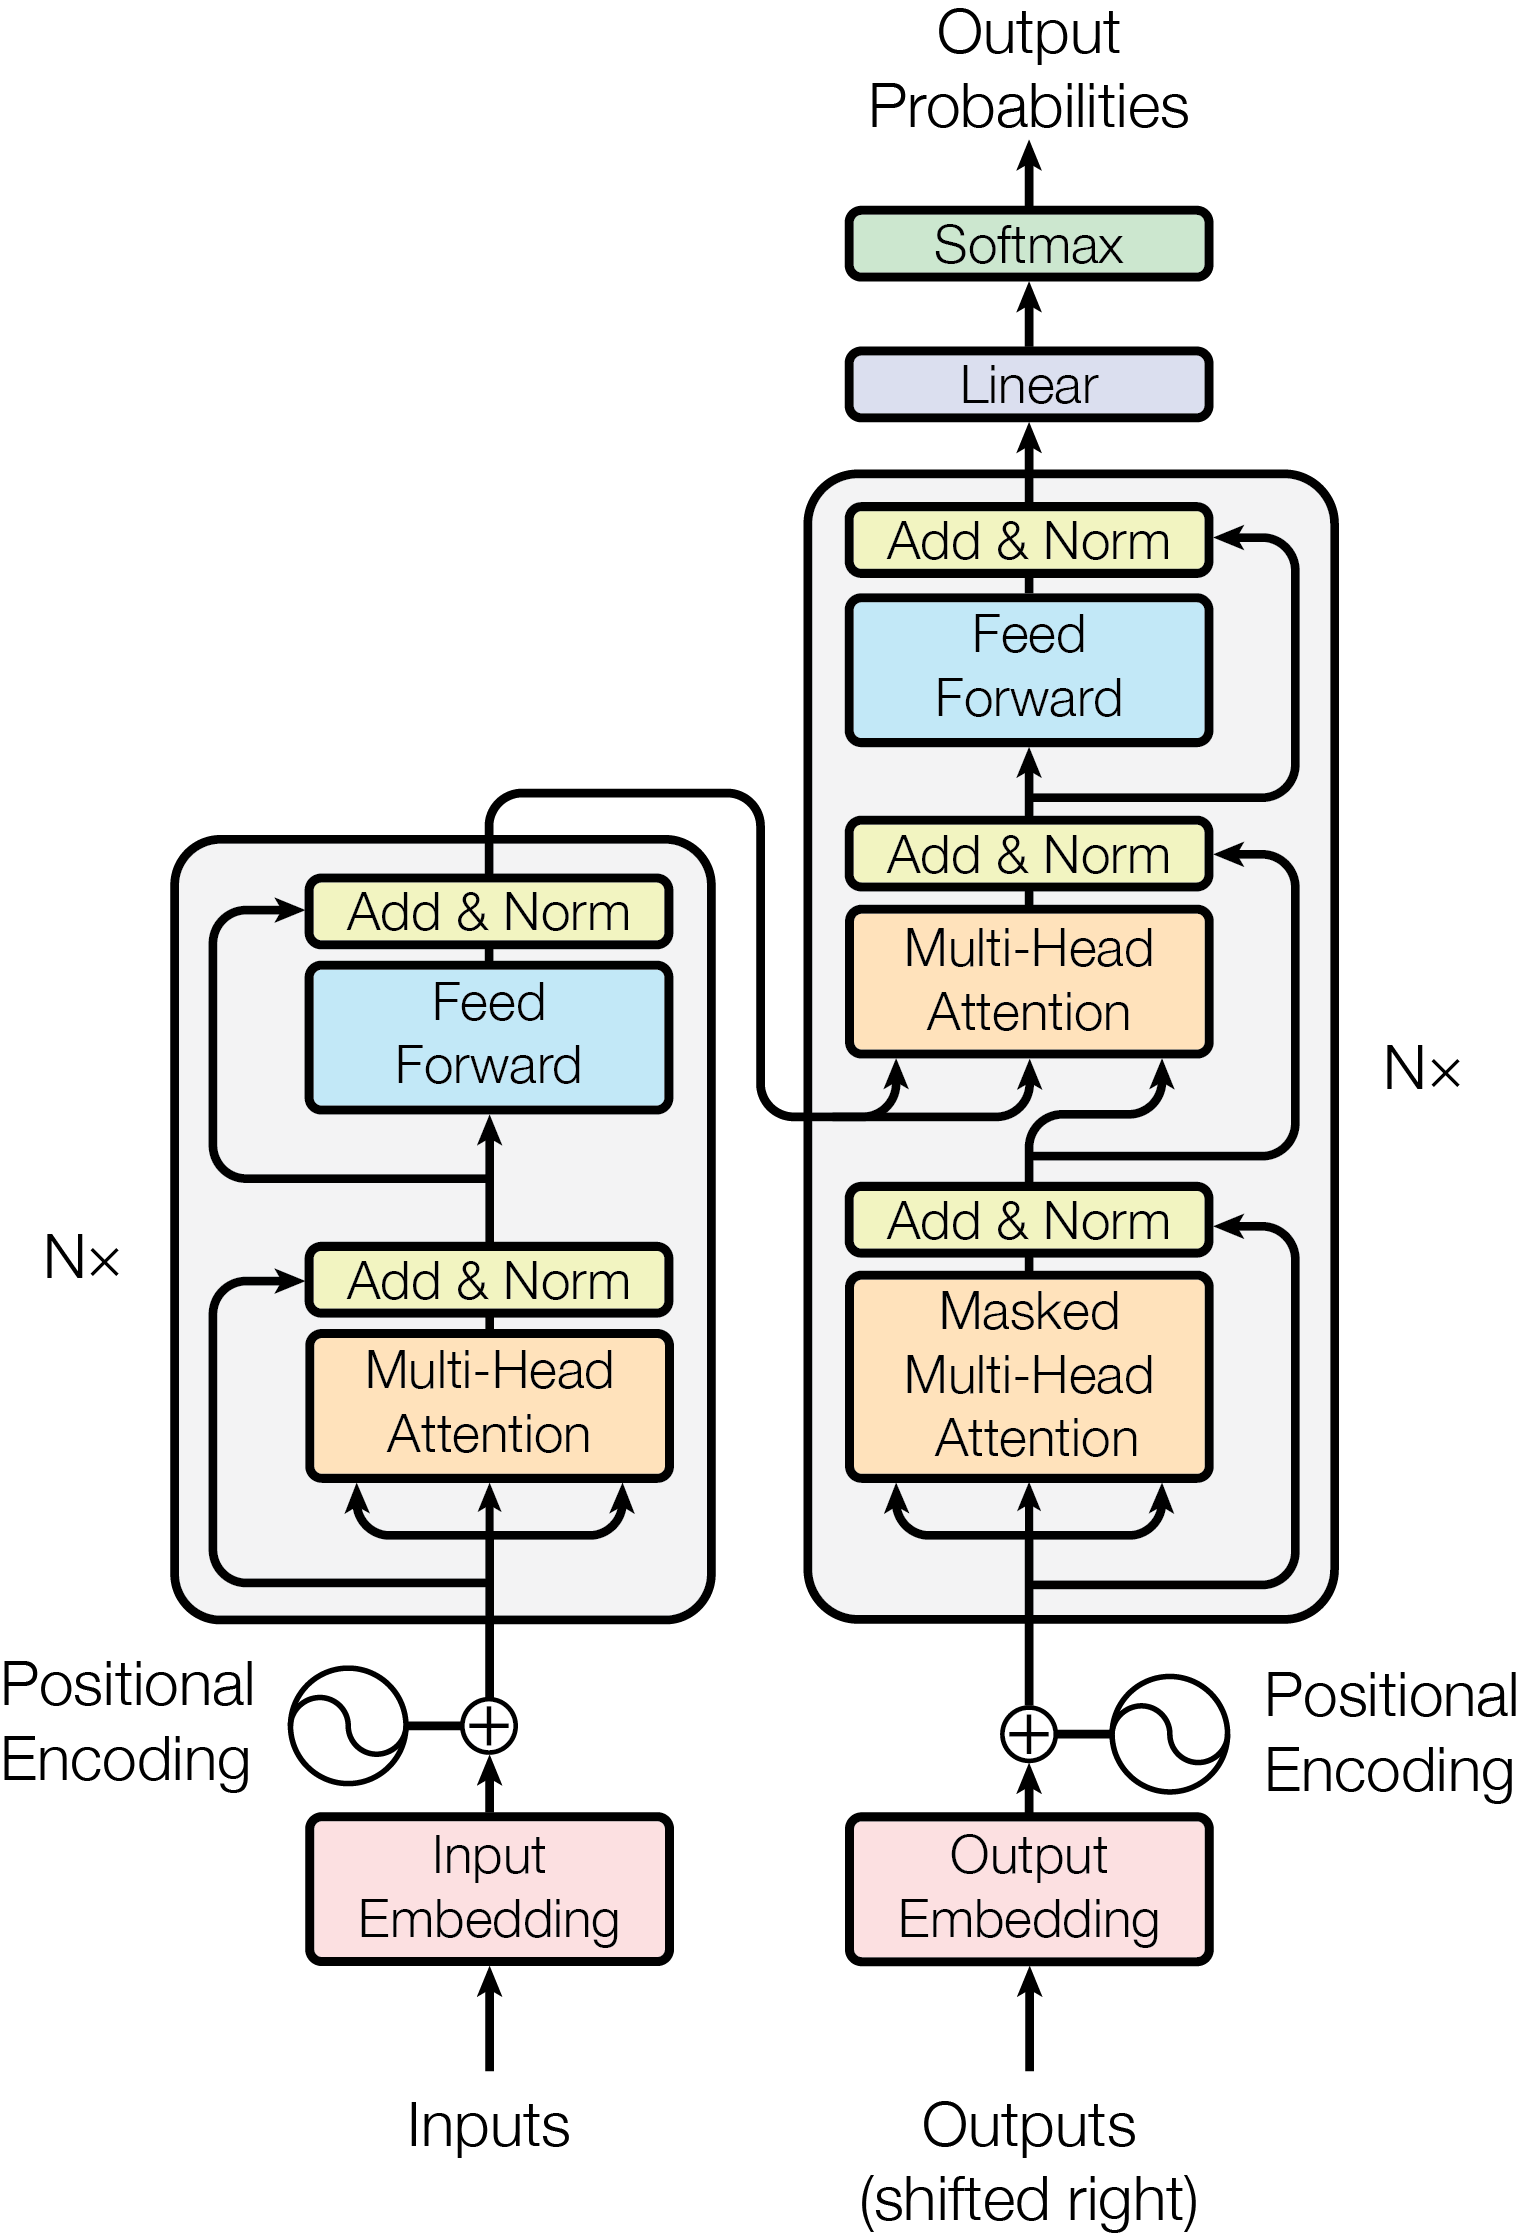
\includegraphics[width=0.5\textwidth]{images/Transformer_Vaswani-et-al2027.png}
        \caption{Illustration du modèle Transformer proposé par \cite{vaswani_attention_2017}}
        \label{fig:transformer}
    \end{figure}
    
    
    
    \subsection{Architecture du modèle Transformer}
    
    Le modèle Transformer suit la structure \emph{encodeur-décodeur}. La partie encodeur capte les informations importantes de l'entrée et la couche décodeur déduit et construit la sortie. L'encodeur et le décodeur ont chacun une couche propre qui est répétée $N$ fois.
    
    Une couche d'encodeur commence par un \emph{mécanisme d'auto-attention multi-tête} (voir sous-section~\ref{ssec:mecattention}). C'est le module "Multi-Head Attention" sur la Figure~\ref{fig:transformer}.  Il est suivi d'une \emph{connexion résiduelle}  dont le résultat est \emph{normalisé}. Une \textbf{connexion résiduelle} correspond à l'ajout de l'entrée d'un module (ici le mécanisme d'attention multi-tête) à sa sortie. La connexion résiduelle et la normalisation sont matérialisées par le module "Add\&Norm" dans la Figure~\ref{fig:transformer}. Le résultat obtenu passe alors dans un \emph{réseau de neurones} composé de deux couches ("Feed Forward" sur la Figure~\ref{fig:transformer}) puis on applique une \emph{connexion résiduelle} avant une nouvelle \emph{normalisation}. Ce processus est répété $N$ fois.
    
    Une couche de décodeur se compose d'un \emph{mécanisme d'attention multi-tête masqué}, d'une \emph{connexion résiduelle} puis d'une \emph{normalisation}. Un \emph{mécanisme d'auto-attention multi-tête} prend en suite en entrée ce résultat ainsi que la sortie des $N$ couches de  l'encodeur. On applique une \emph{connexion résiduelle} sur la sortie puis le tout est \emph{normalisé} avant de passer dans un \emph{réseau de neurones} de deux couches, de subir une nouvelle \emph{connexion résiduelle} puis d'être \emph{normalisé} une fois de plus. Ce processus aussi est répété $N$ fois.
    
    Avant d'entrer dans l'encodeur, l'entrée est encodée. On parle d'\emph{embedding}. On lui ajoute un \emph{encodage positionnel} pour identifier la position de chaque composant dans l'entrée. Ces opérations sont aussi appliquées à la sortie obtenue par le modèle lorsqu'elle est fournie en entrée du décodeur.
    
    
    \subsection{Mécanisme d'attention}
    \label{ssec:mecattention}
    
    L'outil central de l'architecture Transformer est le \emph{mécanisme d'auto-attention multi-tête}. C'est une variante du mécanisme d'attention.
    
    Le \textbf{mécanisme d'attention} est une opération composante à composante qui souligne le lien des composants d'une entrée entre eux \cite{morgan_explainable_2023}.  Mathématiquement, cette opération correspond à un produit de matrices. Plus précisément, le mécanisme d'attention décrit par \cite{vaswani_attention_2017}, appelé \textbf{scaled dot-product attention} et illustré dans la Figure~\ref{fig:scaledDotProduct}, correspond à un produit de matrices associées à un équilibrage (scaling) et une pondération:
    
    \begin{align*}
        \text{Attention}(Q,K) &= \text{softmax}(\frac{QK^T}{\sqrt{d_h}})\\
        \text{Output}(Q,K,V) &= \text{Attention}(Q,K)V\\
    \end{align*}
    
    
    $Q$, $K$ et $V$ sont des matrices de dimension $d_h\times n$ appelées \emph{Query}, \emph{Key} et \emph{Value}. Elles correspondent respectivement aux informations recherchées, aux informations dont on dispose et aux informations que l'on peut communiquer \cite{morgan_explainable_2023}. La matrice $\text{Attention}(Q,K)$ est appelée \textbf{matrice d'attention}. Elle représente la façon dont chaque mot est lié aux autres $n$ mots de l'entrée et l'importance de ce lien.
    
    Parfois, les matrices $Q$, $K$ et $V$ sont issues de la même donnée. Dans ce cas, le mécanisme d'attention est appelé \textbf{auto-attention}. C'est une forme très utilisée du mécanisme d'attention.
    
    
    Dans leur modèle, \cite{vaswani_attention_2017} projettent les données en entrée du mécanisme d'attention dans $h$ sous-espaces de dimension $d_h$, appliquent le mécanisme d'attention sur chaque projection puis concatènent les sorties obtenues avant de reprojeter dans un nouvel espace. Ces projections et espaces sont appris lors de l'entraînement. On appelle cette variante \textbf{le mécanisme d'auto-attention multi-tête}. Si l'attention et l'auto-attention  (illustré dans la Figure~\ref{fig:scaledDotProduct}) peuvent être vus comme une unité neuronale, le mécanisme d'attention multi-tête (voir Figure~\ref{fig:multi-head-attention}) est comparable à une couche de neurones.
    
    Dans certains usages, les composants d'une entrée ne doivent porter attention qu'aux composants qui les précèdent. Par exemple, lorsqu'on cherche à construire une phrase, on ignore les mots qui se situent après celui qu'on est en train de construire. On ne peut donc pas prendre en compte ces mots dans la construction. Les \textbf{mécanisme d'attention masqués} répondent à ce besoin. Les coefficients de la matrice d'attention correspondant à de l'attention portée par un mot vers un successeur sont remplacés par $-\infty$. Dans le cas du \emph{scaled dot-product attention}, ce processus de masquage est effectué après le scaling (division par $\sqrt{d_h}$) mais avant l'application de softmax. 
    % \alh{ici j'aurais inversé le 3.1.1 et 3.1.2. pour aller du plus gros grain au plus fin. , voire mettre le mécanisme d'attention comme un focus dans le 3.1.2. }
    
    \begin{figure}
        \parbox{7cm}{%
        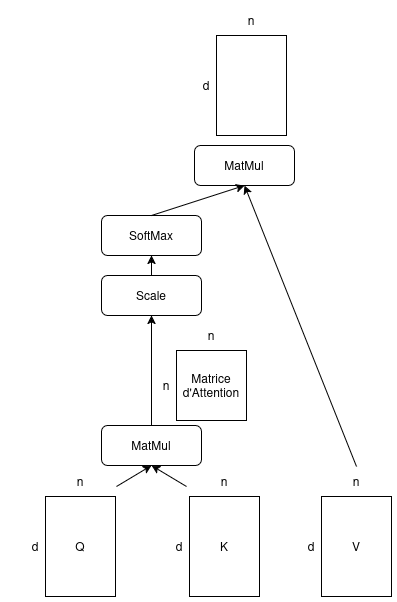
\includegraphics[width=0.4\textwidth]{images/Illustration_Rapport_S9-scaledDotProdAttention.png}
        \caption{Illustration du \emph{scaled dot-product} issu du modèle Transformer \cite{vaswani_attention_2017}}%
        \label{fig:scaledDotProduct}}%
        \qquad
        \begin{minipage}{7cm}%
        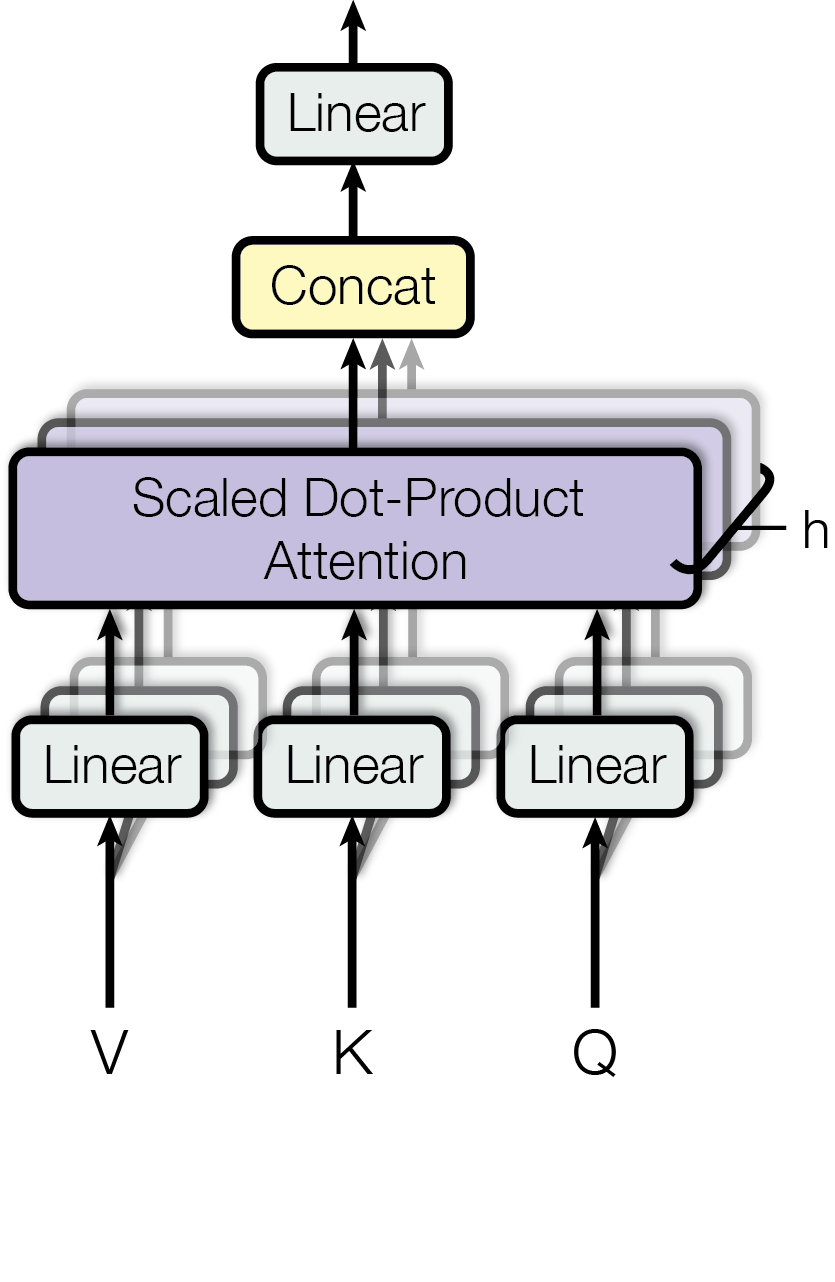
\includegraphics[width=0.8\textwidth]{images/MultiHeadAttention_Vaswani-et-al2017.png}
        \caption{Illustration du \emph{mécanisme d'auto-attention multi-tête} proposé par \cite{vaswani_attention_2017}}%
        \label{fig:multi-head-attention}%
        \end{minipage}%
    \end{figure}
    
    
    
    \subsection{Des modèles à base de Transformer pour l'analyse d'image}
    
    Dans le domaine de l'analyse et du traitement automatique de l'image, les modèles les plus répandus sont basés sur les réseaux de neurones convolutionnels. Le mécanisme d'attention est parfois intégré à ces modèles pour permettre une meilleure performance. \cite{dosovitskiy_image_2021} propose un modèle pour la classification d'images qui n'exploite pas de CNN mais se base exclusivement sur l'architecture Transformer et le mécanisme d'attention.
    
    Le \textbf{Vision Transformer}, illustré par la Figure~\ref{fig:VisionTransformer}, traite les images en les découpant en morceaux appelés \textbf{patches}. Ces parties sont encodées puis complétées par un embedding positionnel. L'ensemble des tokens obtenus est complété d'un token de classification \texttt{[CLS]} puis passé à un encodeur de Transformer. Le token \texttt{[CLS]} ne dépend pas de l'entrée mais à la sortie de l'encodeur, sa représentation reflète l'intégralité de l'image. La représentation du token \texttt{[CLS]} est en suite passée dans un petit réseau de neurones qui classe l'image. 
    
    
    \begin{figure}
        \centering
        \includegraphics[width=\textwidth]{images/ViT_Dosovitskiy-et-al2021.pdf}
        \caption{Illustration Vision Transformer proposé par \cite{dosovitskiy_image_2021}}
        \label{fig:VisionTransformer}
    \end{figure}
    
    
    \subsection{Des modèles à base de Transformer pour le traitement de la langue naturelle}
    
    Le modèle Transformer de \cite{vaswani_attention_2017} a inspiré plusieurs modèles de langue basés sur cette architecture. 
    
    \cite{radford_improving_2018} propose un modèle basé sur la partie \emph{décodeur} du modèle Transformer. L'architecture du modèle GPT (\emph{Generative Pre-Training}), illustré par la Figure~\ref{fig:gpt}, est composée de $N=12$ itérations du bloc décodeur. Les blocs décodeur sont composés d'un \emph{mécanisme d'auto-attention multi-tête masqué} associé à une \emph{connexion résiduelle} suivie d'une \emph{normalisation} puis d'un \emph{réseau de neurone} avec une \emph{connexion résiduelle} encore une fois suivie d'une \emph{normalisation}. L'enchaînement de blocs décodeur est précédé d'un \emph{encodage} des composants de l'entrée associés à un \emph{encodage positionnel}.\\
    Au delà de l'architecture utilisée par \cite{radford_improving_2018}, la méthode d'entraînement joue un rôle important dans la performance du modèle GPT. Dans un premier temps, le modèle est \emph{pré-entraîné} d'une façon présentée comme \emph{non-supervisée} sur un très grand corpus de texte pour apprendre une représentation universelle de son environnement. Après cela, le modèle est affiné à l'aide de données étiquetées qui correspondent à la tâche tierce attribuée au modèle: on parle de \textbf{fine-tunning}. 
    
    \begin{figure}
        \centering
        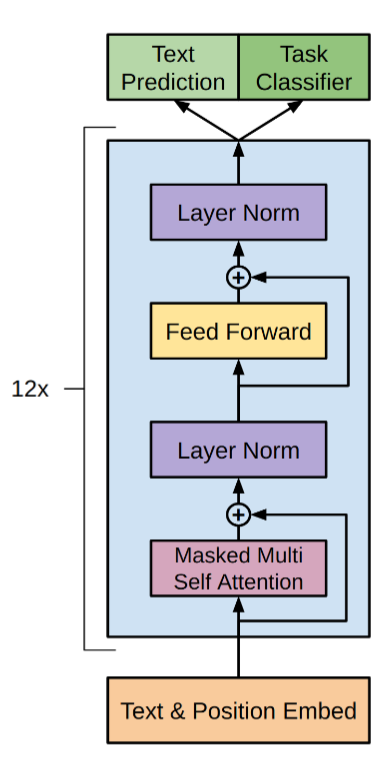
\includegraphics[width=0.3\textwidth]{images/GPT_Radford-et-al2018.png}
        \caption{Illustration du modèle GPT proposée par \cite{radford_improving_2018}}
        \label{fig:gpt}
    \end{figure}
    
    Un autre modèle basé sur le modèle Transformer est le \emph{Bi-directional Encoder Representations from Transformer} (BERT) proposé par \cite{devlin_bert_2019}. Contrairement au modèles GPT, il se base sur un \emph{encodeur} de Transformer et non pas un décodeur. Ainsi, il utilise des \emph{mécanismes d'attention} qui ne sont pas masqués. Comme pour le modèle GPT, le modèle BERT et entraîné en deux temps. Une représentation globale de l'environnement est d'abord apprise de façon \emph{semi-supervisée} à l'aide de deux tâches: prédire les tokens masqués dans une entrée et prédire la phrase suivant celle donnée en entrée. Le modèle est en suite \emph{fine-tunné} avec des données étiquetées issues d'un dataset spécialisé pour la tâche visée.\\
    Depuis la publication de \cite{devlin_bert_2019}, le modèle BERT a été repris et adapté pour de multiples usages. En effet, au delà de ses bonnes performances et de sa forte polyvalence, sa méthode d'entraînement rend sa spécialisation facile. Plusieurs travaux ont été effectués sur la spécialisation du modèle \cite{aftan_survey_2023}. On retrouve un certain nombre de modèles basés sur BERT spécialisés dans une langue cible comme le français \cite{segonne_jargon_2024, martin_camembert_2020}, le néerlandais \cite{delobelle_robbert_2020} ou l'arabe \cite{antoun_arabert_2021}. D'autres modèles sont conçus pour les \emph{langues de spécialité} : dans des contextes techniques tels que la justice \cite{douka_juribert_2021} ou la médecine \cite{lee_biobert_2020}, on attend d'un modèle qu'il soit capable de s'exprimer avec un vocabulaire ou des codes précis et spécifiques à ce contexte. Au delà des travaux d'application, on retrouve aussi des versions améliorées du modèle initial comme \cite{sanh_distilbert_2020} qui propose un modèle aussi efficace mais avec moins de paramètres ou tel que \cite{wahab_dibert_2021} qui intègre d'autres compétences linguistiques telles que des notions de syntaxe. 
    
    Nous nous limitons ici aux modèles de la forme encodeur ou décodeur comme BERT et GPT. D'autres formes de modèles inspirés du modèle Transformer existent \cite{touvron_llama_2023, raffel_exploring_2020}. Certains modèles prennent la forme d'un décodeur ou d'un encodeur, d'autres exploitent les deux parties. 
    
    
\section{Modèles boite-noire}

    Comme mentionné précédemment, les modèles et systèmes cherchent à extraire une représenta\-tion d'un environnement afin de répondre à une tâche. Selon la technologie sur laquelle se base un modèle, la représentation sous-jacente de son environnement est plus ou moins accessible. Cela peut être dû à la complexité technique de l'algorithme d'apprentissage ou à la complexité du modèle en lui-même (calculs lourds, grand nombre de paramètres) \cite{garouani_investigating_2024}. \\
    À l'inférence, le processus décisionnel suivi n'est pas transparent pour tous les modèles. La procédure est connue mais il n'est pas toujours possible de lui donner du sens d'un point de vue humain. Les modèles pour lesquels les mécanismes internes de décision sont obscures et/ou difficiles à comprendre sont appelées des \textbf{modèles boite-noire} \cite{bell_its_2022, garouani_investigating_2024}.\\
    Parmi ces modèles, on retrouve les modèles de deep-learning tels que les réseaux de neurones (DNN, CNN, RNN,...), les modèles Transformer ou encore les méthodes telles que \emph{Random Forest} \cite{garouani_investigating_2024}.



\chapter{Expliquer les modèles boite-noire}
    Dans le chapitre précédent, nous avons constaté que la plupart des modèles couramment utilisés sont des modèles boite-noire. Pour autant, ces modèles peu explicables pourraient être exploités dans certains secteurs nécessitant une confiance et une interprétation de ses outils. Afin de permettre cette utilisation, des méthodes ont été mises en place pour essayer d'extraire leurs enjeux internes. On présente dans ce chapitre leurs différentes familles accompagnées d'exemples et on évoque les enjeux autour du développement de ces techniques. On se situe ici dans le domaine de l'\emph{explicabilité post-hoc}.
    
    Dans cette partie, on fera la confusion entre \emph{modèle} et \emph{système}. Dans le cas des modèles, la sortie correspond à la représentation de la donnée produite par le modèle.
    
\section{Taxonomie des méthodes d'explication}
    Pour mettre en évidence des liens entre les entrées et les sorties des modèles boite-noire, de nouvelles méthodes sont régulièrement mises en place. On parle de \emph{méthode d'explication} ou \emph{d'explicabilité}.
    
    Dans la littérature, on retrouve plusieurs critères qui distinguent les méthodes d'explicabilité. Certains modèles cherchent à fournir une explication du fonctionnement du modèle pour n'importe quelle entrée. On parle d'explication \textbf{globale}. Par opposition, on trouve des méthodes qui cherchent à lier les éléments d'une entrée avec la sortie obtenue par le modèle en se concentrant sur une entrée. L'explication n'est pas vraie en général mais seulement pour l'entrée étudiée. C'est une méthode d'explication \textbf{locale}.\\
    Les méthodes d'explication se distinguent aussi par leur manière de procéder. Certaines méthodes, dites \textbf{model-agnostic}, ne s'intéressent pas aux paramètres du modèle mais uniquement à son comportement sur les entrées. À contrario, les méthodes \textbf{model-specific} cherchent à exploiter les paramètres du modèle pour aider à donner une explication. Cela a pour conséquence qu'elles ne sont pas exploitables pour tous les modèles.\\
    Dans le cas de la classification, certaines méthodes proposent une explication différente pour chaque classe de la sortie. Ces méthodes sont dites \textbf{class-specific}. Quand l'explication est commune à toute les classes, on parle de méthode \textbf{class-agnostic}.
    
    Selon la stratégie utilisée par les méthodes, ont peu les séparer en plusieurs familles parmi lesquelles ont retrouve :
    \begin{itemize}
        \item les méthodes basées sur la \emph{perturbation} des entrées
        \item les méthodes basées sur la \emph{rétro-propagation} d'information dans le modèles
        \item les méthodes basées sur le \emph{gradient}
        \item les méthodes basées sur les \emph{matrices d'attention}
        \item les méthodes basées sur l'étude d'\emph{exemples} bien choisis
    \end{itemize}
    
    Ces familles ainsi que des exemples de méthode sont présentés dans la partie suivante.
    
    Les différentes caractéristiques des méthodes d'explication sont récapitulées dans les Figures~\ref{fig:taxoXAIMeth} et \ref{fig:recapPropXAIMeth}.
    
\begin{figure}
    \centering
    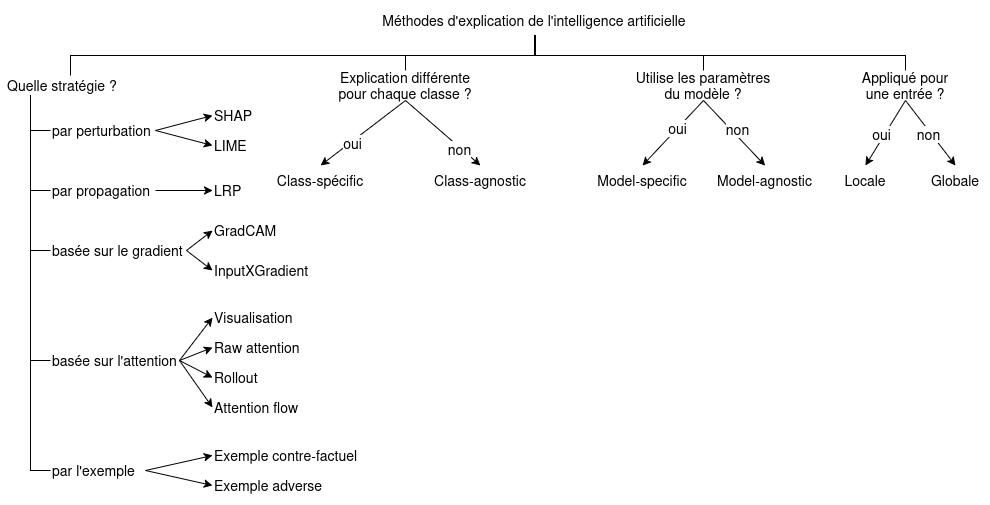
\includegraphics[width=\textwidth]{images/Illustration_Rapport_S9-TaxonomieMethodeXAI.drawio.png}
    \caption{Taxonomie des méthodes d'explication de l'intelligence artificielle incluant les méthodes présentées dans la Section~\ref{sec:XAIMeth}}
    \label{fig:taxoXAIMeth}
\end{figure}

\begin{figure}
    \centering
    \begin{tabular}{|l||c|c||c|c||c|c|}
        \hline
        Famille de méthodes & locale & globale & model-specific & model-agnostic & class-specific & class-agnostic \\
        \hline
        par perturbation & $\times$ &      &                & $\times$      &                & $\times$  \\
        par rétro-propagation & $\times$ & & $\times$       &               & $\times$      &           \\
        basée sur gradient & $\times$   &  & $\times$       &               & $\times$      &           \\
        basée sur l'attention & $\times$&  & $\times$       &               &               & $\times$  \\
        par l'exemple & $\times$ &         &                & $\times$      &               & $\times$\\
        \hline
        
    \end{tabular}
    \caption{Tableau récapitulatif des propriétés des familles de méthodes d'explicabilité présentées dans ce chapitre}
    \label{fig:recapPropXAIMeth}
\end{figure}

\section{Les méthodes d'explication répandues}
    \label{sec:XAIMeth}

    \subsection{Méthodes basées sur la perturbation}
        
        Les \textbf{méthodes d'explication par perturbation} cherchent à déduire une explication de la prédiction $M(x)$ pour une entrée $x$ et un modèle $M$ en observant les prédictions $M(x')$ associées à des entrées $x'$ proche de $x$. L'idée est, à l'aide des prédictions $M(x')$ pour des versions perturbées de $x$, de mettre en évidence les caractéristiques de $x$ qui contribuent à la prédiction $M(x)$. 
        
        La méthode LIME (Local Interpretable Model-agnostic Explanations) \cite{molnar_interpretable_2025, ribeiro_model-agnostic_2016} cherche à simplifier le modèle boite-noire $M$ par un modèle explicable $M'$ qui approxime $M$ au voisinage de l'entrée $x$. Pour cela, LIME:
        \begin{enumerate}
            \item Créé un ensemble $X$ d'entrées $x'$ qui sont des versions de $x$ perturbées
            \item Récupère la prédiction $M(x')$ du modèle qu'on cherche à expliquer pour chaque entrée $x'$
            \item Entraîne un modèle interprétable $M'$ (voir Section~\ref{mod_interpretables}) à l'aide de ces prédictions en les pondérant par la proximité de $x'$ à $x$
            \item Considère l'interprétation de $M'$ comme une explication de la contribution des éléments de $x$ dans sa prédiction $M(x)$
        \end{enumerate}
        Cette méthode est \emph{locale}, \emph{model-agnostic} et \emph{class-agnostic}.
        
        La méthode SHAP (SHapley Additive exPlanations) \cite{molnar_interpretable_2025, lundberg_unified_2017} cherche à attribuer à chaque élément de $x$ une contribution à la différence entre $M(x)$ et la moyenne des toutes les prédictions. À l'aide d'une base de donnée similaire à celle produite avec la méthode LIME, on calcule la contribution de chaque attribut de $x$ à sa prédiction. Une contribution peut être positive ou négative. La somme des contributions des attributs correspond à la différence entre $M(x)$ et la moyenne des prédictions. SHAP est aussi une méthode \emph{locale}, \emph{model-agnostic} et \emph{class-agnostic}.\\

    \subsection{Méthodes basées sur la rétro-propagation}
        
        Les \textbf{méthodes d'explication basées sur la rétropropagation} vise à propager une grandeur couche par couche à travers un réseau de neurones de la sortie vers l'entrée (c'est à dire en sens inverse). Pour une couche donnée, on obtient la contribution de donne issue de ce noeud dans la prédiction. En particulier, lorsqu'on atteint l'entrée du modèle, on obtient une contribution pour chaque composante pour une entrée donnée. Ces méthodes se basent sur la Deep Taylor Decomposition \cite{montavon_explaining_2017} : 
        
        $$\left\{
        \begin{array}{rl}
            R^{(n)}_j &= \mathcal{G}(X,W,R^{(n+1)}) = \sum_{i}X_j\frac{\partial L_i^{(n)}(X,W)}{\partial X_j}\frac{R_i^{(n+1)}}{L_i^{(n)}(X,W)} \quad \forall 0< n <N\\
            R_j^{(N)} &= \mathbb{1}_{t}(j) \text{ $t$ est la classe étudiée}
        \end{array}\right.
        $$
        $n$ représente la couche du réseau, $j$ représente le neurone dans la couche, $X$ est la sortie de la $n^e$ couche et $W$ est la matrices des poids entre les couches $n$ et $n+1$. La valeur $R_j^n$ correspond à la quantité d'information, appelée \emph{importante}, dans le $j^e$ noeud de la $n^e$ couche du réseau. $\mathbb{1}_{t}$ est l'indicatrice de $t$ : $\mathbb{1}_{t}(t) = 1$ et $\forall x\not= t\; \mathbb{1}_{t}(x) = 0$
        
        Dans le cadre des réseaux de neurones profonds avec la fonction d'activation ReLU effectuant une classification, \cite{montavon_layer-wise_2019} propose la méthode Layer-wise Relevance Propagation (LRP).\\
        Pour une entrée $x$, chaque attribut $j$ reçois un coefficient $R_j^0$ indiquant l'importance de l'attribut dans le calcul de la probabilité de la classe $t$. On l'obtient en remontant couche par couche depuis la sortie. $R^N$ est le vecteur avec que des 0 sauf à la $t^e$ classe qui vaut 1. La formule pour remonter le réseau est :
        $$
        R^{(n)}_j = \mathcal{G}(X^+, W^+, R^{(n+1)}) = \sum_i \frac{x_j^+ w_{ji}^+}{\sum_{j'} x_{j'}^+ w_{j'i}^+} R_i^{(n+1)}
        $$
        où $v^+ = max(0,v)$
        
        Ces méthodes sont \emph{locales}, \emph{model-specific} et \emph{class-specific}.
        
    \subsection{Méthodes basées sur le gradient}
        
        Les \textbf{méthodes d'explication à base de gradient} \cite{ancona_gradient-based_2019} suivent une intuition similaire à celle des méthodes basées sur le rétro-propagation : raisonner depuis la sortie du modèle vers son entrée. Ce qui distingue ces deux familles de méthode est le sens associé à la propagation et la grandeur propagée. Les méthodes à base de gradient construisent une fonction au fur et à mesure de cette propagation. En effet, ces méthodes se basent sur le calcul \textbf{gradient des sorties du modèle en fonction des entrées}. Cela donne une approximation linéaire de l'impact de chaque partie de l'entrée sur chaque valeur en sortie.\\
        Formellement, si on défini un modèle réseau de neurones comme une fonction $M$ qui associe à une entrée $(x^0_1,\dots,x^0_{N_0})$ une sortie $(y_1,\dots,y_{N_C})$ et qu'on note $(x^i_1,\dots,x^i_{N_i})$ les $N_i$ coefficients obtenus au cours du passage dans la $i^\text{ème}$ couche du modèle, le gradient de la sortie $y_j$ est 
        $$\nabla_{(x^0_i)_i}y_j = \left( \frac{\partial y_j}{\partial x^0_1}, \dots, \frac{\partial y_j}{\partial x^0_{N_0}} \right)$$
        et est obtenu à l'aide de  
        $$\forall i \in \{1,\dots, N_l\} \forall j \in \{1,\dots, N_C\}, \, \frac{\partial y_j}{\partial x^i_{N_l}} = \sum_{k=0}^{N_{i+1}} \frac{\partial y_j}{\partial x^{i+1}_{k}} \frac{\partial x^{i+1}_{k}}{\partial x^i_{N_l}}$$
        
        Ces méthodes dépendent de l'entrée étudiée, explore les paramètres du modèle qui est un réseau de neurones (éventuellement convolutif) : elles sont \emph{locale}, \emph{model-specific} et \emph{class-specific}.
        
        Certaines méthodes associent le gradient de la sortie en fonction de l'entrée avec d'autres outils pour fournir une explication. La méthode GradCAM \cite{selvaraju_grad-cam_2017} associe le calcul du gradient avec l'approche Class Activation Mapping (CAM) pour obtenir une "carte d'influence" dans le cadre des modèles ayant pour environnement des images. La méthode Input$\times$Gradient \cite{shrikumar_not_2017} multiplie le gradient obtenu par l'entrée. 
        
        \begin{tcolorbox}[colback=blue!5!white,
                      colframe=blue!75!black,
                      title=Gradient à l'entraînement et lors de l'explication
                     ]
            Il faut distinguer le gradient utilisé lors de l'entraînement du modèle et celui utilisé pour fournir une explication. Lors de l'entraînement d'un modèle, on exprime le gradient des sorties \textbf{en fonction des paramètres}. Dans ce cas, les calculs intermédiaires effectués dans les noeud d'un réseau de neurones sont des coefficients et les paramètres sont les variables de la fonction. Il est généralement noté $\nabla_{(W_i,b_i)_i}y_j$ où les $W_i$ et $b_i$ sont les matrices de paramètres et les biais du modèle.\\
            Lors de l'explication d'un modèle, on observe le gradient des sorties \textbf{en fonction des entrées}. Les paramètres du modèle sont des simples coefficients et les composantes de l'entrée sont des variables. On le note $\nabla_{(x_i)_i}y_j$ où les $x_i$ sont les composantes de l'entrée.
        \end{tcolorbox}

    
    \subsection{Méthodes basées sur l'attention}
        
        Comme expliqué précédemment, le mécanisme d'attention produit et exploite une matrice d'attention qui exprime le lien des composantes de la donnée en entrée entre elles. Les \textbf{méthodes d'explication basées sur l'attention} exploitent ces informations pour déduire une explication sur le processus de décision suivi par le modèle sur l'entrée appliquée.
        
        Une première façon d'exploiter les matrices d'attention obtenues lors de l'inférence sur une entrée est la visualisation. Des outils tels que BertViz \cite{vig_multiscale_2019} proposent une interface de visualisation des coefficients des matrices d'attention. Observer ces matrices permet notamment de trouver de potentiels biais ou d'identifier les mécanismes d'auto-attention et les têtes de mécanisme d'auto-attention multi-tête les plus importants.
        
        Les matrices d'attention peuvent aussi être plus ou moins traitées pour en extraire des "cartes d'influence". Une façon très simple est de visualiser la carte obtenue à partir d'une seule matrice d'attention. La méthode raw attention \cite{chefer_transformer_2021} visualise la "carte d'influence" extraite de la matrice d'attention issue du mécanisme d'attention le plus proche de la sortie du modèle.
        
        \cite{abnar_quantifying_2020} propose deux méthodes d'extraction de scores à partir des matrices d'attention issues d'un modèle. Ces méthodes cherchent à exploiter toutes les matrices d'attention obtenues lors d'une inférence. Elles se basent sur l'interprétation des matrices d'attention comme des représentations de graphes. Ces deux méthodes se différencient par la façon dont les différentes matrices d'attention (et par extension les arêtes des graphes) interagissent.\\
        La première méthode appelée \emph{rollout attention} voit le passage de l'information comme le parcours d'un chemin. Si on note $A_i$ la matrice représentant les matrices d'attention du bloc $i$, on cherche $\tilde{A}_N$ la matrice de scores recherchée où $N$ est le nombre de blocs dans le modèle et on l'obtient à l'aide de l'expression :
        
        $$\tilde{A}_i = \left\{\begin{array}{ll}
        A_i & \text{si } i = 0\\
        A_i\tilde{A}_{i-1} & \text{sinon}
        \end{array}\right.
         $$
        
        La méthode \emph{attention flow} fait le parallèle entre le passage de l'information et le problème de flot dans les graphes. La matrice de score associée à une entrée sur un modèle correspond au flot maximal du graphe.
        
       Ces méthodes sont \emph{locales}, \emph{model-specific} et \emph{class-agnostic}
        
    
    \subsection{Méthodes basées sur les exemples}
        
        Les \textbf{méthodes d'explication basées sur les exemples} cherchent à mettre en évidence des informations sur le modèle étudié à l'aide de données exemples construites ou issues de la base de données disponible.
        
        Les \textbf{exemples adverses} visent à mettre le modèle en difficulté. Il sont construits à partir d'entrées bien traitées (correctement classées ou avec une bonne prédiction) qui sont perturbées de telle manière que la différence soit peu voir indiscernable pour l'humain mais que le modèle ne soit plus capable de bien la traiter \cite[Chap~30]{molnar_interpretable_2025}. La Figure~\ref{fig:adversarialExample} montre un exemple de construction d'exemple adverse.\\
        Les exemples adverses sont utilisés dans le cadre de l'explicabilité pour le perfectionnement des modèles. Ils mettent en évidence les faiblesses du modèle et sont parfois utilisés en complément de la base de donnée originale pour augmenter la résistance du modèle à des attaques similaires.
        
        \begin{figure}
            \centering
            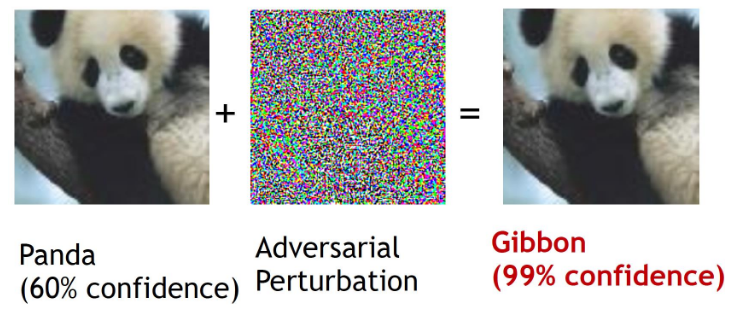
\includegraphics[width=0.5\textwidth]{images/AdversarialPerturbation_Panda.png}
            \caption{Donnée perturbée pour construire un exemple adverse}
            \label{fig:adversarialExample}
        \end{figure}
        
        Un autre type d'exemple utilisé pour expliquer les modèles sont les \textbf{exemples contre-factuels} \cite[Chap~15]{molnar_interpretable_2025}. Ces exemples cherchent à illustrer un lien de causalité entre la perturbation d'une entrée et la sortie obtenue. Cette causalité n'est pas nécessairement cohérente avec le contexte mais souligne le changement de sortie fournie par le modèle entre les deux versions de l'entrée. De tels exemples sont obtenus en cherchant à atteindre une certaine prédiction à partir d'une entrée fixée qui sera perturbée. Une perturbation pertinente vérifie plusieurs critères : peu de composantes de l'entrée sont modifiées, les modifications sont aussi faibles que possible, la prédiction erronée recherchée est atteinte et l'entrée perturbée est plausible. On note que plusieurs perturbations peuvent vérifier toutes ces conditions et qu'elle peuvent même se contredire. Dans ce cas, il est possible de toute les présenter ou d'en sélectionner qu'une partie à l'aide des critères définis plus tôt. 
        
        Ces méthodes sont \emph{locales}, \emph{model-agnostic} et \emph{class-agnostic}.


\section{Évaluer les méthodes d'explication}
    Que ce soit pour juger la qualité d'une méthode d'explication ou pour faire un choix parmi plusieurs méthodes, il est nécessaire de pouvoir comparer les méthodes d'explication. Évaluer et comparer les méthodes d'explication n'est pas un travail simple et de nouveaux frameworks et de nouvelles métriques sont encore proposés. On s'intéresse ici aux enjeux de l'évaluation des méthodes d'explicabilité, aux métriques et aux méthodes de comparaison.
    
    \subsection{Ce qu'on attend d'une explication}
    \label{ssec:attendus}
%    \begin{comb}
%    De façon générale on attends (rappel)\\
%    - que la méthode reflète le raisonnement du modèle (réponde à pourquoi)\\
%    - quelle soit humainement accessible\\
%    Concrètement / plus précisément:\cite{mersha_evaluating_2025} \\
%    - robuste : ne pas être trop sensible aux petits change et dans une entrée\\
%    - conscistente : entre deux modèles similaires, les explication soient aussi similaire pour une même entrée\\
%    - contrastante : pointe des élémnts qui font que ça change / des explications similaires ont des sortie simialires / des explications très opposées ont des sorties différentes\\
%    Des éléemnts qui porent à débat:\\
%    - jugement humain de l'explication : qualitatif donc pb de comparaison
%    Des exigences qui dépendent de l'usage \cite{bell_its_2022}:
%    - dépends du public visé\\
%    - dépends de l'usage A SOURCER\\
%    \end{comb}
    
    Par la définition d'explication, on attend d'une méthode d'explication qu'elle fournisse des explications qui soient humainement accessibles tout en reflétant le plus possible le mécanisme de décision du modèle. Concernant les méthodes d'explication elles-mêmes, \cite{mersha_evaluating_2025} présente plusieurs critères attendus d'une méthode d'explication:
    \begin{description}
        \item[Robustesse] : Les explications fournies pour deux entrées très similaires doivent elles aussi être similaires.
        \item[Consistance] : Une méthode appliquée à deux modèles similaires et entraînés sur les mêmes données doit proposer des explications similaires sur une même entrée (voir Figure~\ref{fig:consistanceMersha-et-al2025}).
        \item[Contraste] : Les explications fournies permettent de marquer le contraste entre deux entrées ayant des prédictions différentes. 
        %\item[Adéquation au raisonnement humain] : Les explications obtenues sont similaires aux explications humaines fournies sur une entrée dont la sortie est connue.
    \end{description}
    Pour chacun de ces critères, \cite{mersha_evaluating_2025} propose une métrique. Une analyse de la correspondance entre ces critères et les métriques proposées serai une piste de poursuite intéressante à ce sujet.
    
    \begin{figure}
        \centering
        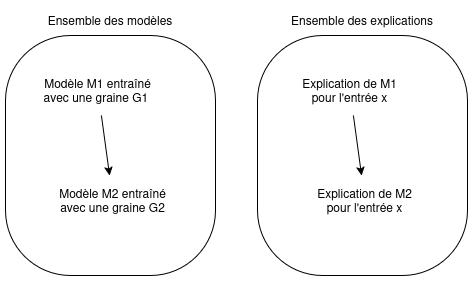
\includegraphics[width=0.7\textwidth]{images/ConsistanceMersha-et-al2025.drawio.png}
        \caption{Une méthode d'explication est consistante si, d'un modèle à l'autre, entraînés sur les mêmes données, elle fourni des explications pour une même entrée dont la différence est comparable à la différence des modèles.}
        \label{fig:my_label}
    \end{figure}
    
    D'autres critères proposés dans la littérature sont plus problématiques. \cite{chefer_transformer_2021} et \cite{mersha_evaluating_2025} mesurent dans leur expérience l'adéquation des explications fournies au raisonnement humain. Cet attendu n'en est pas un concernant les méthodes d'explicabilité car ces dernières doivent être fidèles au modèle et non raisonnement humain. Par contre, l'adéquation au raisonnement humain peut être un attendu concernant les modèles dans l'optique de leur donner un comportement et/ou un raisonnement plus humain. C'est une piste étudiée dans la Section~\ref{sec:modelesconcepts}.\\
    Par ailleurs, \cite{neely_song_2022} interroge la notion d'explication idéale. Ainsi, il devient difficile de définir un protocole de comparaison des méthodes d'explication (entre elles ou avec une explication de référence) qui puisse faire consensus.
    
    D'autre part, un récapitulatif des attendus proposés dans la littérature permettrait de dégager un éventuel manque dans la liste précédente.
    
    
    
    
    \subsection{Les métriques}
%    \begin{comb}
%    \cite{chefer_transformer_2021} propose mesure d'adéquation au modèles avec le "Pointing Game"\\
    
%    Les problématiques rencontrées avec les métriques:\\
%    - qualitatif vs quantitatif\\
%    - manque de métriques reconnues\\
%    - biais humain : la machine ne pense pas tjrs comme humin ~> on ne peut pas comparer explication et GoundTruth\\
%    - comparabilité des explications issues de méthodes différentes (format)
%    \end{comb}
    
    
    Au delà de l'absence de consensus sur les critères définissant une bonne méthode d'explication, \cite{garouani_investigating_2024} souligne la rareté des métriques quantitatives qui couvrent l'ensemble des critères et qui soit adaptées à plusieurs modèles. \cite{mersha_evaluating_2025} insiste aussi sur l'absence de consensus concernant les métriques.
    
    Par ailleurs, certaines métriques sont remises en question. \cite{gilpin_explaining_2019} dénonce l'évalua\-tion des explications à l'aide du jugement humain. On fourni une entrée, sa sortie pour un modèle et l'explication obtenue par la méthode d'explication étudiée à un évaluateur humain chargé de juger plusieurs critères. Au-delà de la difficulté d'organiser une telle évaluation, cette dernière est sujette aux biais en faveur de l'intelligibilité et en défaveur de la fidélité au modèle. De plus, elle n'est pas quantitative non plus, ce qui pose problème pour comparer les méthodes d'explication entre elles.
    
    
    Une métrique adaptée pour mesurer la fidélité des explications fournies par une méthode d'explication est celle utilisée par \cite{chefer_transformer_2021}. Cette dernière mesure la proximité de l'explication au raisonnement du modèle à l'aide d'une méthode de perturbation. Les composants de l'entrée jugés importants par l'explication sont masqués. On observe la performance du modèle sur ces nouvelles entrées. Si elle baisse drastiquement, cela signifie que les composants en question sont effectivement importants dans le processus de décision du modèle. 
    
    %\alh{on s'attend un peu à voir votre position sur tout ceci}
    
%    \begin{comb}
%    Pour comparer on a des exigences en plus sur les métriques:\\
%    - quantitatif\\
%    - compatible avec plusieurs méthodes et nature de données\\
%    - equitable : cpte bien les compétences de toutes les métriques\\
    
    
%    \cite{mersha_evaluating_2025} énumère des exigences et propose un framework:\\
%    - Complexité du modèle\\
%    - Nature des entrées\\
%    - Données elles-même\\
%    - Nature de la tâche demandée\\
%    - Méthodes d'explicabilité\\
%    - Métriques pour l'explicabilité
%    \end{comb}
    
    Lorsqu'il s'agit d'utiliser des métriques pour comparer des méthodes d'explication, certains problèmes sont accentués. En plus de devoir permettre une comparaison, les métriques doivent être adaptées à plusieurs méthodes et contextes. \\
    \cite{mersha_evaluating_2025} énumère plusieurs exigences pour concevoir un protocole d'évaluation et de comparaison de méthodes d'explication: Une grande diversité est nécessaire pour obtenir un avis global sur les méthodes. Ce besoin de diversité porte sur la complexité du modèle, la nature des entrées, la variété des tâches, les thématiques des entrées, les méthodes d'explication comparées, les attendus et les métriques utilisées,...
    %\alh{c'est une mine, c'est vraiment interessant !}
    

\chapter{Des modèles explicables}
Jusqu'ici, nous nous sommes intéressés à l'\emph{explicabilité post-hoc}, ses outils, les besoins auxquels elle répond et les difficultés rencontrées. Un autre axe de l'explicabilité est l'\emph{explicabilité by-design}. L'objectif n'est plus de retrouver le raisonnement une fois le modèle ou le système construit mais de concevoir des modèles et systèmes qui soient plus interprétables.

\section{Modèles Interprétables simples}
    \label{mod_interpretables}
    
    Il existe des modèles et méthodes de construction de modèles qui sont moins complexes que les réseaux de neurones profonds ou les méthodes ensemblistes. Parmi ces méthodes, on retrouve les arbres de décision, les modèles basés sur la régression linéaire ou encore les méthodes à base de listes de règles \cite[Chapitres~6 à 11]{molnar_interpretable_2025}. Ces formes de modèles permettent d'exprimer de façon logique et/ou mathématique les éléments pris en compte pour obtenir une sortie ou une autre.\\
    Ces modèles sont réputés pour la facilité avec laquelle on peut accéder au processus de décision appliqué lors d'une prédiction. Les modèles transparents sont souvent qualifiés de \textbf{modèles interprétables}. 
    
    
\section{Des compromis inhérents aux attendus d'une explication}
    \label{sec:tradesoff}
    Construire des solutions pour favoriser l'explicabilité en intelligence artificielle engendre certaines confrontations. À première vue, concernant l'explicabilité by-design, il faudrait choisir entre la performance des modèles et leur interprétabilité. De la même manière, du coté de l'explicabilité post-hoc, le sentiment de devoir choisir entre fidélité au modèle et accessibilité au grand public est présent.
    
    \subsection{Compromis entre performance des modèles et interprétabilité}
%    \begin{color}{gray}
%    Une autre caractéristique qui les oppose aux modèles boite-noire est la performance. En effet, si les modèles boite-noire sont réputés pour leurs bonnes performances, on reproche souvent aux arbres de décision, aux modèles linéaires et aux modèles à base de règle leur faible performances par rapport au modèles de deep learning. On notera tout de même que si cette intuition semble évidente, l'idée que l'interprétabilité d'un modèle soit inversement proportionnelle à sa performance ne semble pas documenté dans la littérature.En ça, Les modèles interprétables sont facilement opposés aux modèles boite-noire présentés précédemment. 
%    \end{color}
    
%    \begin{comb}
%    On constate les boites-noires performantes d'un coté et les modèles interprétables inadaptés à certaines tâches (manipulation du texte par exemple SOURCER)\\
%    Il n'y a pas de publications en ce sens pourtant \\
%    \cite{rudin_stop_2019} dénonce même cette idée en la qualifiant d'illusion (RETROUVER LE PASSAGE)
%    \end{comb}
    
    Les modèles boite-noires tels que les réseaux de neurones et les Transformers sont réputés pour leurs bonnes performances sur une très grande diversité de tâches. Face à ces modèles boite-noire, les modèles interprétables réputés pour leur transparence peinent à faire valoir leurs performances pourtant similaires sur certaines tâches. La simplicité des représentations assimilées par ces modèles est facilement décriée. De plus, ces performances tendent à réduire lorsque la tâche appliquée et l'environnement associé se complexifient. De ce constat naît l'idée que les notions d'interprétabilité et de performance sont inversement proportionnelles. Cependant, il est important de noter qu'il n'y a pas de consensus allant dans ce sens. \cite{johansson_trade-off_2011} montre que cette relation existe entre les modèles à base de décision (arbres et listes de décision) et les modèles ensemblistes (\emph{Random Forest}) pour les tâches de classification dans le contexte bio-pharmaceutique alors que \cite{rudin_stop_2019} dénonce cette idée en la qualifiant de mythe. Ce débat encourage les travaux cherchant à maintenir l'interprétabilité des modèles tout en augmentant leurs performances. 
    
    
    \subsection{Compromis entre fidélité des explications et accessibilité pour le grand public}
%    \begin{color}{gray}
%    Cependant, certains auteurs tels que \cite{bell_its_2022} mettent en garde sur le sens de cette interprétabilité. Si ces modèles s'expriment bien à l'aide le la logique et des mathématiques, il est toujours possible de remettre en question la légitimité de ces expressions \cite{molnar_interpretable_2025}: Représentent-elles bien l'environnement?, Peut-on parler d'interprétabilité pour un arbre de décision de profondeur 15?  \\
%    \end{color}
    
%    \begin{comb}
%    \cite{gilpin_explaining_2019} expose le besoin de choix entre fidélité au modèle et intelligibilité du modèle\\
%    \cite{molnar_interpretable_2025} remet en question interprétabilité des modèles dits interprétables (DT de hauteur 15)\\
%    cela fait écho au problème du public visé :\\
%    - \cite{bell_its_2022} : le grand public ne sait pas se servir des explications\\
%    - \cite{kastner_relation_2021} : les explications rendent digne de confiance MAIS ne font pas la confiance du grand public (qui se rendent compte des faiblesses)
%    \end{comb}
    
    En explicabilité post-hoc, on construit des méthodes qui fournissent des explications concernant les processus de décision des modèles boite-noire. On attend d'une explication qu'elle reflète le raisonnement du modèle tout en étant humainement intelligible. \cite{gilpin_explaining_2019} souligne l'importance de faire un bon compromis entre la fidélité au modèle d'une explication et son intelligibilité. Simplifier de façon excessive peut créer des explications persuasives induisant une confiance indue de l'utilisateur pour le modèle. \\
    \cite{molnar_interpretable_2025} remet aussi en question la réelle interprétabilité des modèles dits interprétables. Est-il légitime de dire d'un arbre de décision de profondeur 20 qu'il est interprétable? La formule le représentant est-elle toujours humainement intelligible?
    
    La sous-section~\ref{ssec:def_expl} pointe la question du public visé par l'explication. \cite{bell_its_2022} et \cite{kastner_relation_2021} se sont intéresses au cas du grand public. \cite{bell_its_2022} pointe le faible impact de l'explication sur la compréhension des décisions des modèles par le grand public. \cite{kastner_relation_2021} met aussi en évidence la nuance entre donner confiance (trust) et mériter la confiance (fiabilité) (trustability dans l'article). Les explications cherchent à mettre en évidence la fiabilité des modèles. Sachant qu'il est rationnel d'avoir confiance dans les modèles fiables, les explications devraient permettre d'avoir  confiance dans les modèles qui méritent cette confiance. Cependant, cette idée n'est pas vérifiée pour le cas du grand public. \cite{kastner_relation_2021} montre que dans ce cas, utiliser les explications n'impacte pas la confiance voire provoque une baisse de celle-ci : cela s'expliquerait par la prise de conscience que les modèles et systèmes d'intelligence artificielle sont faillibles ou par la difficulté du grand public à comprendre ces explications.
    
    Si les méthodes d'explication actuelles ne semblent pas répondre au besoin d'explicabilité pour le grand public, d'autres pistes du coté de l'explicabilité by-design sont explorées à travers les modèles neuro-symboliques (Section~\ref{sec:neuro-symbolique}) et les modèles à base de concepts (Section~\ref{sec:modelesconcepts}).

\section{Les modèles neuro-symboliques}
\label{sec:neuro-symbolique}
    
    Bien que l'exploitation des méthodes explication soient remise en question par \cite{bell_its_2022} et \cite{kastner_relation_2021} en ce qui concerne le grand public (voir la Section~\ref{sec:tradesoff}), les spécialistes et les concepteurs en IA restent très intéressés par ce qui se passe dans les modèles boites-noires. La possibilité de mettre en évidence des biais et la miniaturisation des modèles motivent aussi les travaux sur l'explicabilité de l'intelligence artificielle.
    %\alh{ne serait-ce que pour des besoins de maintenabilité}. 
    Ainsi, de nombreux travaux portent sur le design de nouveaux modèles qui malgré une allure de modèle boite-noire, seraient plus interprétables. Ces modèles cherchent à tirer parti des méthodes symboliques et/ou interprétables en les associant à des structures plus complexes basées sur les réseaux de neurones. On les appelle \textbf{modèles neuro-symboliques} \cite{bhuyan_neuro-symbolic_2024}. \\
    Au-delà de leur interprétabilité et leur transparence, les modèles symboliques sont appréciés pour leur application stricte de la logique sur laquelle ils se basent. Lorsque les entrées sont correctement identifiées, ces modèles ont de bons résultats. Les réseaux de neurones sont reconnus pour leur capacité à apprendre des comportements dont les motivations sont plus difficiles à cerner et reproduire un comportement moins rationnel plus difficile à formuler à l'aide des modèles symboliques. Sur la base de ces constats, l'idée de les associer permettrait de profiter des points forts de chacun : exploiter la précision des raisonnements logiques des modèles symboliques tout en profitant de l'intuition des réseaux de neurones. Pour cela, on retrouve différentes façons des les associer. \cite{bhuyan_neuro-symbolic_2024} distingue plusieurs familles, nous les listons ici sans détailler plus leurs spécificités
    % \alh{, nous les listons ici sans détailler plus avant leurs spécificités(Mme Dao sera friande de ce paragraphe : ) donc prémunissons nous contre des attentes non satisfaites qui ne sont pas le sujet de cet état de l'art)}
    :\\
    La première forme, désignée par \emph{symbolic-neuro-symbolic}, regroupe les modèles composés d'un enchaînement d'applications de méthodes symboliques et connexionnistes (à base de réseaux de neurones). \\
    Les modèles de la forme \emph{symbolic[neuro]} sont utilisés de la même façon que les méthodes symboliques. Ce qui les distingue est que les prédicats et fonctions sont des petits réseaux de neurones.\\
    La famille de modèles \emph{neuro $\mid$ symbolic} correspond aux modèles qui font collaborer les deux approches. On retrouves des systèmes tels que celui proposé par \cite{kalouli_hy-nli_2020}. Un modèle se base sur la logique naturelle, le second est un BERT. Un troisième modèle est entraîné pour déterminer lequel des deux premiers est le plus susceptible de fournir la bonne sortie en fonction de caractéristiques choisies et détectées par ces deux modèles. \\
    La quatrième famille proposée est la famille \emph{neuro-symbolic $\rightarrow$ neuro}. Ces modèles, qui sont des réseaux de neurones, sont conçus et/ou entraînés à l'aide de concepts et techniques symboliques. Dans cette famille, on retrouve les modèles qui exploitent l'injection de connaissances \cite{ciatto_symbolic_2024}.\\
    Les modèles de la famille \emph{neuro$_{\text{symbolic}}$ } sont des modèles connexionnistes entraînés à l'aide de fonctions de perte particulières. Elles forcent l'assimilation de connaissances sous forme symbolique en incluant des contraintes logiques.\\
    Enfin, les modèles de la forme \emph{neuro[symbolic]} intègrent des opérations logiques à l'échelle des couches du réseau de neurones qui les constituent. Au lieu d'effectuer une produit matriciel pour passer d'une couche à l'autre, c'est une opération logique qui est effectuée.
    
    Si ces modèles contiennent bien des notions et des outils symboliques, il reste pertinent de questionner la nature explicable de ces derniers. En effet, lors de l'assimilation par le modèles des outils symboliques, il n'est pas impossible que ces derniers perdent en transparence. De plus, les formules symboliques restent des concepts techniques et ne sont pas nécessairement accessibles à tous les public. Ainsi, l'approche neuro-symbolique semble être une piste intéressante aussi bien du point de vue de la performance que de l'explicabilité. Cependant, ces buts doivent être gardés à l'esprit lors de la conception afin de ne pas complexifier des modèles sans que cela n'apporte de gain.
    % \alh{L'investigation de ces approches semblent être une piste de poursuite interessante... ou un truc du genre ? le pavé n'est pas indigeste en tout cas !}
    
    
    
\section{Modèles à base de concepts}
\label{sec:modelesconcepts}

    La plupart des méthodes d'explication post-hoc fournissent des explications sous la forme de contributions de chaque composant de l'entrée à travers des réels ou des "cartes d'influence". C'est à l'utilisateur de comprendre le sens associé à ces éléments. Ce travail n'est pas toujours évident ni accessible à l'utilisateur \cite{poursabzi-sangdeh_manipulating_2021}.\\
    Les modèles interprétables disposent d'une méthode définie pour exprimer leur structure sous forme de formule mathématique ou logique. Encore une fois, si la formule est facile à obtenir, il n'est pas nécessairement simple de la lire ni de lui donner du sens. Dans le cas des méthodes neuro-symboliques, la présence de structures symboliques dans le modèle accorde une plus grande transparence au modèle mais son intelligibilité peut rester problématique pour les mêmes raisons.
    
    Les \textbf{modèles à base de concepts} s'attaquent à la problématique de l'intelligibilité du raisonnement sous-jacent dans les modèles. Au lieu d'injecter dans le modèle des règles parfois abstraites, on cherche à lui apprendre des concepts humainement intelligibles. Un \textbf{concept} est défini par \cite[Chap.~29]{molnar_interpretable_2025} comme "n'importe quelle abstraction, telle qu'une couleur, un objet ou même une idée".  \cite{poeta_concept-based_2023} distingue plusieurs types de concepts : Les \emph{concepts symboliques}  correspondent aux concepts humains tels que "bleu", "oiseau", "manger",...  Les \emph{concepts non-supervisés} sont appris par la machine de façon non supervisée. Certains éléments capturés sont intelligibles mais ce n'est pas toujours le cas de tous. Les \emph{prototypes} sont des concepts représentés par des exemples. Les \emph{concepts textuels} sont des descriptions de concepts sous forme de texte.
    
    Les modèles à base de concepts peuvent prendre plusieurs formes \cite{poeta_concept-based_2023}:
    \begin{itemize}
        \item Les \emph{modèles à base de concepts supervisés} sont entraînés à reconnaître des concepts choisis. Les données d'entraînement sont annotées avec les concepts qui lui sont associés. Une couche interne du réseau est entraînée pour les reconnaître en parallèle de l'entraînement du système pour la tâche tierce. Si on ne dispose pas de données d'entraînement annotées pour les concepts, un autre lot de données peut être utilisé après l'entraînement à la tâche pour superviser l'apprentissage des concepts.
        \item Les \emph{modèles à base de concepts non supervisés} sont entraînés sur des données qui ne sont pas annotés pour les concepts. L'apprentissage des concepts est forcé à l'aide d'une fonction d'apprentissage adaptée. Ainsi, les n\oe uds désignés par la fonction d'apprentissage assimileront des concepts non-supervisés de façon autonome.
        \item Les \emph{modèles hybrides} sont à mi chemin entre les deux types de modèles précédents : une partie des neurones est entraînée à l'aide des données annotés et une autre partie apprend des concepts non-supervisés.
        \item Les \emph{modèles génératifs} fournissent eux-même une représentation des concepts nécessaires. Ceux-ci sont alignés avec la représentation obtenue de l'entrée, ce qui permet de conclure sur la sortie du modèle. Par exemple, un modèle de langue interne au modèles génère une description des classes possibles en sorties. Elles sont alors encodées afin d'être comparées avec la représentation extraite de l'entrée (par exemple une image). Le modèle génératif s'appuie sur le comparaison de ses deux informations pour classer l'entrée. 
    \end{itemize}

    La particularité des modèles à base de concepts nous permet d'espérer une plus grande transparence et accessibilité du raisonnement impliqué lors de l'utilisation du modèle \cite{poeta_concept-based_2023}. Au delà de l'objectif d'explicabilité, \cite{kim_interpretability_2018, kim_help_2023} espèrent que les raisonnements appris et adoptés par ces modèles soient plus proche du raisonnement humain dans le sens où ils ne seraient pas seulement corrélés mais une reproduction de celui-ci. Cependant, il faut noter que forcer les modèles actuels à raisonner comme des humains revient à contraindre leur apprentissage. Cela alors même que ces modèles ne sont pas des reproductions exactes du cerveau humain mais des outils inspirés de l'idée de neurone. Par conséquent, on peut craindre une difficulté pour ces modèles à atteindre les performances attendues. 
    
 


\chapter{Explicabilité pour le traitement de la langue}

    Comme expliqué précédemment, les grands modèles de langue (LLM) tels que BERT et GPT sont des modèles d'intelligence artificielle boite noire. Au-delà de la complexité de l'association de leurs composants, ces modèles contiennent un très grand nombre de paramètres ce qui rend leur comportement opaque. Cette opacité des LLM est critique dans certains contextes (santé, légal,...), ce qui explique le besoin d'utiliser des méthodes d'explication pour ces modèles. Dans ce chapitre, on s'intéresse aux modèles de langue qui sont utilisés pour les problèmes impliquant des entrées et/ou sortie sous forme de texte en langue naturelle ainsi qu'aux méthodes d'explicabilité appliquées dans ces cas.
    
    \section{Enjeux autour des méthodes d'explicabilité pour le NLP}
        \subsection{Généralités}
        Les méthodes d'explication présentées dans les chapitres précédents peuvent être appliquées aux LLMs comme à n'importe quel autre modèle ou système. Cependant, \cite{mersha_evaluating_2025} pointe le fait qu'une grande partie d'entre-elles n'ont pas été conçues spécifiquement pour les LLMs et que les explications obtenues ne sont pas toujours aussi fidèles ou adéquates qu'attendu.
        % \alh{c'est à dire ? comme nous le verrons peut suffir} Les méthodes en question nécessitent une adaptation. 
        La conception de nouvelles méthodes pensées spécialement pour les LLM est même présentée comme urgente dans cet article. 
        
        Au-delà du caractère adapté ou non des méthodes d'explicabilité génériques, leur scalabilité est aussi remise en question par \cite{garouani_investigating_2024} qui pointe notamment la complexité en temps très importante de l'application des méthodes basées sur SHAP \cite{marzouk_tractability_2024}. 
        
        D'un point de vue empirique, certains résultats de travaux sur les méthodes d'explication laissent penser que les performances de ces méthodes dépendent de la tâche et/ou du modèle auquel on l'applique. \cite{chefer_transformer_2021} présente les résultats de sa méthode appliquée à des données visuelles et textuelles. On obtient des "cartes d'influence" qui semblent moins satisfaisantes pour les données textuelles que pour les images (voir la Figure~\ref{fig:textchefer}. Au delà de ce cas, il ne semble pas exister d'étude comparative des performances d'une méthode d'explication sur différentes tâches avec des entrées textuelles et non textuelles. 
        %\alh{voilà un sujet qui trouverait sa place en conclusion et comme proposition de semestre 2 par exemple}
        
        \subsection{Cas des méthodes à base d'attention}
        Parmi les méthodes évoquées précédemment, on retrouve les méthodes basées sur l'attention. Elles sont très répandues dans ce domaine car la majeure parties des modèles utilisent le mécanisme d'attention comme technologie principale. De plus, au delà de l'extraction des matrices d'attention, l'intuition associée à ce mécanisme laisse présager des explications fidèles et intelligibles. 
        
        Cependant, les évaluations de ces métriques ne sont pas toujours aussi encourageantes. \cite{mersha_evaluating_2025} obtient une très faible adéquation entre explications humaines et celles obtenues par visualisation de l'attention. Ces méthodes sont même remises en question (voir sous-section~\ref{ssec:attendus}. \\
        D'un point de vue technique,  \cite{chefer_transformer_2021} souligne le fait que n'exploiter que les matrices d'attention revient à ignorer le reste du modèle c'est-à-dire se priver de composants tout aussi importants que le mécanisme d'attention lors de la construction de l'explication recherchée. Cette publication propose de comparer les prédictions de plusieurs méthodes avec celle issue d'une méthode en combinant plusieurs (voir Figure~\ref{fig:textchefer}). D'un point de vue théorique, \cite{lopardo_attention_2024} incite même à mettre de coté l'idée d'exploiter les matrices d'attention comme outil d'explicabilité de l'IA. Son analyse mathématique d'un petit modèle à base d'attention montre que ces matrices capturent moins d'éléments que des méthodes telles que SHAP \cite{lundberg_unified_2017}.
        
        \begin{figure}
            \centering
            \includegraphics[width=\textwidth]{images/0_neg_1.pdf}
            \caption{Exemple de comparaison proposée par \cite{chefer_transformer_2021}. Cette entrée est un commentaire négatif bien classé par le modèle utilisé. Les explications proposées sont (dans l'ordre) la sélection humaine des mots importants (Ground Truth), l'explication pour la méthode proposée pour la classe négatif (N), l'explication pour la méthode proposée pour la classe positif (P), l'explication de Partial LRP pour la classe N, l'explication de Partial LRP pour la classe P, l'explication de GradCAM pour la classe N, l'explication de GradCAM pour la classe P, l'explication de LRP pour la classe N, l'explication de LRP pour la classe P, l'explication de raw attention et l'explication de rollout.}
            \label{fig:textchefer}
        \end{figure}
        
    \section{Enjeux autour des métriques d'évaluation de ces explications}
        Face aux critiques portées sur les méthodes d'explicabilité appliquées au NLP, on retrouve des critiques concernant les méthodes et les métriques d'évaluation de ces dernières.\\
        \cite{neely_song_2022} montre que juger une explication en observant sa corrélation avec celles fournies par des méthodes à attribution (famille d'explication qui regroupe les méthodes à base de gradient, de rétro-propagation de pertinence et à base de perturbation) n'est pas pertinent car les méthodes à attribution elles-mêmes ne sont pas corrélées entre elles.\\
        \cite{mersha_evaluating_2025} remet en question la capacité des métriques à base de perturbation à estimer l'efficacité des méthodes d'explications lorsqu'elles sont appliquées à de très grands modèles.
        
\chapter{Conclusion}
    
    Dans ce rapport et au cours de mon immersion, nous avons vu comment fonctionnent les modèles actuels tels que les modèles basés sur le Transformer et constaté que leur complexité et leur grand nombre de paramètres engendrent une grande opacité. Cette nature de modèle boite-noire est problématique dans certains domaines où il est incontournable de pouvoir accéder aux raisons motivant l'obtention d'une certaine sortie ou d'un certain comportement. \\
    Ce besoin de transparence peut être traité de deux façons. La première stratégie est de construire des méthodes qui, en observant le modèle ou son comportement, peuvent donner des indications humainement intelligibles sur les raisons de son comportement ou sa sortie. Ces méthodes se basent sur différentes stratégies et il reste encore difficile de les comparer et de déterminer les tâches et contextes pour lesquels elles sont le plus adaptées. La seconde stratégie vise à construire de nouveaux modèles qui soient transparents tout en restant capables de traiter les mêmes tâches avec la même performance. Il n'est pas simple de construire de tels modèles car même si des outils interprétables sont utilisés lors de leur construction, ce n'est pas pour autant qu'ils restent interprétables lors de l'usage.\\
    Dans le contexte du traitement automatique de la langue, on retrouve les mêmes problématiques. Celles-ci sont d'autant plus présentes que les méthodes d'explication ne sont pas toujours aussi efficaces dans ce contexte que dans le cas général et que les métriques d'évaluation ne sont pas toujours adaptées.
    
    Les difficultés rencontrées en explicabilité de l'intelligence artificielle pour le traitement de la langue naturelle mettent en évidence que de nombreuses études et perspectives sont encore possibles. \\
    Dans un premier temps, une étude comparative des méthodes d'explication appliquées aux données textuelles et non textuelles (images, tables attribut-valeur, données séquentielles,...) permettrait d'identifier les méthodes d'explication les plus efficaces selon la tâche et le modèle étudié. Cela aidera peut-être à déterminer les besoins de l'explicabilité pour les LLMs qui ne sont pas partagés avec les autres modèles. Ces éléments sont de potentielles pistes pour construire des méthodes d'explication spécifiques aux besoins de l'explicabilité de l'IA pour le NLP. \\
    Dans le domaine de l’évaluation des méthodes d’explication, un récapitulatif des attendus et des métriques existantes pourrait mettre en lumière de potentiels éléments manquants dans ce contexte et de les combler. Par ailleurs, il serait intéressant de questionner la comparabilité des modèles appliqués à des textes et des modèles appliqués à des données non-textuelles. Cela orienterait sur un besoin ou non de méthodes d'explication et de métriques d'évaluation qui soient universelles au sens des tâches et modèles.
    

\chapter{Lexique et acronymes}
\section{Acronymes}

\begin{description}
    \item[CNN (Convolutionnal Neural Network)] : Réseau de Neurones Convolutionnel
    \item[DNN (Deep Neural Network)] : Réseau de Neurones Profond
    \item[IA/ AI (Intelligence Artificielle/ Artificial Intelligence)] : domaine visant à faire adopter à une machine un comportement et/ou un raisonnement rationnel et/ou humain.
    \item[LLM (Large Language Model)] : Grand Modèle de Langue
    \item[ML (Machine Learning)] :  Apprentissage Automatique
    \item[NLP/TALN (Natural Language Processing)] : Traitement Automatique de la Langue Naturelle
    \item[RGPD (Règlement Générale de Protection des Données)] : réglementation établie par l'union européenne sur la gestion des données personnelles
    \item[RNN (Recurrent Neural Network)] : Réseau de Neurones Récurrent
    \item[XAI (eXplainable Artificial Intelligence)] : eXplicabilité pour l'Intelligence Artificielle
\end{description}

\section{Lexique}

\begin{description}
    \item[Boite-noire] : Modèle ou système dont le raisonnement lors d'une prédiction n'est pas transparent ou humainement compréhensible
    \item[Carte d'influence (relevance map)] : Fonction qui à chaque composante (pixel, mot,...) de l'entrée d'un modèle associe un réel reflétant l'importance de ce composant dans le processus de décision du modèle
    \item[Entrée] : Donnée fournie au système lors du processus d'inférence
    \item[Environnement] : Ensemble de données dont est issue l'entrée fournie à un modèle ou un système
    \item[Explicabilité by-design] : méthodes d'explicabilité portant sur la conception de modèles plus transparents 
    \item[Explicabilité post-hoc] : méthodes d'explicabilité portant sur la conception de méthodes d'extraction de relations entre les entrées et les sorties des modèles/systèmes
    \item[Fonction d'apprentissage / fonction de perte] : fonction utilisée pour entraîner le modèle
    \item[Inférence] : Application du modèle/système sur une nouvelle donnée pour obtenir une sortie
    \item[Intelligence artificielle connexionniste] : Partie du domaine de l'intelligence artificielle exploitant les réseaux de neurones.
    \item[Intelligence artificielle symbolique] : Partie du domaine de l'intelligence artificielle portant sur les systèmes experts basés sur des ensembles de règles prédéfinies et des mécanismes de raisonnement logique.
    \item[Modèle] : Représentation d'un environnement
    \item[Paramètre] : Valeur dans le modèle déterminée lors de l'entraînement et utilisée lors du processus de décision. Les grands modèles de langue en contiennent plusieurs centaines de milliers.
    \item[Sortie] : Donnée obtenue par le système à l'issue du processus d'inférence
    \item[Système] : Fonction qui à une entrée associe une sortie en respectant une spécification
\end{description}


\bibliographystyle{apalike}
\bibliography{sample.bib,IAAct.bib}

\end{document}\documentclass{report}

